
%%% Preamble
\documentclass[paper=a4, fontsize=11pt]{scrartcl}

%%AGREG0
\usepackage{float}
%\usepackage{geometry}
%\geometry{verbose,tmargin=2cm,bmargin=2cm,lmargin=2cm,rmargin=2cm,headheight=2cm,headsep=2cm}
%\geometry{verbose,tmargin=2cm,bmargin=2cm,lmargin=2cm,rmargin=2cm,headheight=2cm,headsep=2cm}

\usepackage[T1]{fontenc}
\usepackage{fourier}
\usepackage[utf8]{inputenc}
\usepackage[english]{babel}					% English language/hyphenation

\usepackage[protrusion=true,expansion=true]{microtype}	
\usepackage{amsmath,amsfonts,amsthm} % Math packages
\usepackage[pdftex]{graphicx}	
\usepackage{url}
\usepackage{import}

\usepackage[margin=2cm]{geometry}
\geometry{verbose,tmargin=2cm,bmargin=2cm,lmargin=2cm,rmargin=2cm,headheight=2cm,headsep=2cm}
% %%% Custom sectioning
\usepackage{sectsty}
\allsectionsfont{\normalfont \scshape}


%%% Custom headers/footers (fancyhdr package)
\usepackage{fancyhdr}
\pagestyle{fancyplain}
\fancyhead{}											% No page header
\fancyfoot[L]{}											% Empty 
\fancyfoot[C]{}											% Empty
\fancyfoot[R]{\thepage}									% Pagenumbering
\renewcommand{\headrulewidth}{0pt}			% Remove header underlines
\renewcommand{\footrulewidth}{0pt}				% Remove footer underlines
\setlength{\headheight}{13.6pt}


%%% Equation and float numbering
\numberwithin{equation}{section}		% Equationnumbering: section.eq#
\numberwithin{figure}{section}			% Figurenumbering: section.fig#
\numberwithin{table}{section}				% Tablenumbering: section.tab#


%%% Maketitle metadata
\newcommand{\horrule}[1]{\rule{\linewidth}{#1}} 	% Horizontal rule

%AGREGO PARA EJ 1
\usepackage{graphicx}
\usepackage{color} 
\usepackage[dvipsnames]{xcolor}
\colorlet{purple}{purple}

%/////////////////////////////////// AGREGO PARA EL EJ 2

    \usepackage{geometry} % Required to change the page size to A4
    \geometry{a4paper} % Set the page size to be A4 as opposed to the default US Letter

    \usepackage{mathtools, nccmath}
    
    \usepackage{tikz}
    \usetikzlibrary{matrix,calc}

    %isolated term
%#1 - Optional. Space between node and grouping line. Default=0
%#2 - node
%#3 - filling color
\newcommand{\implicantsol}[3][0]{
    \draw[rounded corners=3pt, fill=#3, opacity=0.3] ($(#2.north west)+(135:#1)$) rectangle ($(#2.south east)+(-45:#1)$);
    }


%internal group
%#1 - Optional. Space between node and grouping line. Default=0
%#2 - top left node
%#3 - bottom right node
%#4 - filling color
\newcommand{\implicant}[4][0]{
    \draw[rounded corners=3pt, fill=#4, opacity=0.3] ($(#2.north west)+(135:#1)$) rectangle ($(#3.south east)+(-45:#1)$);
    }

%group lateral borders
%#1 - Optional. Space between node and grouping line. Default=0
%#2 - top left node
%#3 - bottom right node
%#4 - filling color
\newcommand{\implicantcostats}[4][0]{
    \draw[rounded corners=3pt, fill=#4, opacity=0.3] ($(rf.east |- #2.north)+(90:#1)$)-| ($(#2.east)+(0:#1)$) |- ($(rf.east |- #3.south)+(-90:#1)$);
    \draw[rounded corners=3pt, fill=#4, opacity=0.3] ($(cf.west |- #2.north)+(90:#1)$) -| ($(#3.west)+(180:#1)$) |- ($(cf.west |- #3.south)+(-90:#1)$);
}

%group top-bottom borders
%#1 - Optional. Space between node and grouping line. Default=0
%#2 - top left node
%#3 - bottom right node
%#4 - filling color
\newcommand{\implicantdaltbaix}[4][0]{
    \draw[rounded corners=3pt, fill=#4, opacity=0.3] ($(cf.south -| #2.west)+(180:#1)$) |- ($(#2.south)+(-90:#1)$) -| ($(cf.south -| #3.east)+(0:#1)$);
    \draw[rounded corners=3pt, fill=#4, opacity=0.3] ($(rf.north -| #2.west)+(180:#1)$) |- ($(#3.north)+(90:#1)$) -| ($(rf.north -| #3.east)+(0:#1)$);
}

%group corners
%#1 - Optional. Space between node and grouping line. Default=0
%#2 - filling color
\newcommand{\implicantcantons}[2][0]{
    \draw[rounded corners=3pt, opacity=.3] ($(rf.east |- 0.south)+(-90:#1)$) -| ($(0.east |- cf.south)+(0:#1)$);
    \draw[rounded corners=3pt, opacity=.3] ($(rf.east |- 8.north)+(90:#1)$) -| ($(8.east |- rf.north)+(0:#1)$);
    \draw[rounded corners=3pt, opacity=.3] ($(cf.west |- 2.south)+(-90:#1)$) -| ($(2.west |- cf.south)+(180:#1)$);
    \draw[rounded corners=3pt, opacity=.3] ($(cf.west |- 10.north)+(90:#1)$) -| ($(10.west |- rf.north)+(180:#1)$);
    \fill[rounded corners=3pt, fill=#2, opacity=.3] ($(rf.east |- 0.south)+(-90:#1)$) -|  ($(0.east |- cf.south)+(0:#1)$) [sharp corners] ($(rf.east |- 0.south)+(-90:#1)$) |-  ($(0.east |- cf.south)+(0:#1)$) ;
    \fill[rounded corners=3pt, fill=#2, opacity=.3] ($(rf.east |- 8.north)+(90:#1)$) -| ($(8.east |- rf.north)+(0:#1)$) [sharp corners] ($(rf.east |- 8.north)+(90:#1)$) |- ($(8.east |- rf.north)+(0:#1)$) ;
    \fill[rounded corners=3pt, fill=#2, opacity=.3] ($(cf.west |- 2.south)+(-90:#1)$) -| ($(2.west |- cf.south)+(180:#1)$) [sharp corners]($(cf.west |- 2.south)+(-90:#1)$) |- ($(2.west |- cf.south)+(180:#1)$) ;
    \fill[rounded corners=3pt, fill=#2, opacity=.3] ($(cf.west |- 10.north)+(90:#1)$) -| ($(10.west |- rf.north)+(180:#1)$) [sharp corners] ($(cf.west |- 10.north)+(90:#1)$) |- ($(10.west |- rf.north)+(180:#1)$) ;
}

%Empty Karnaugh map 4x4
\newenvironment{Karnaugh}%
{
\begin{tikzpicture}[baseline=(current bounding box.north),scale=0.8]
\draw (0,0) grid (4,4);
\draw (0,4) -- node [pos=0.7,above right,anchor=south west] {y2 y1} node [pos=0.75,below left,anchor=north east] {w y3} ++(135:1);
%
\matrix (mapa) [matrix of nodes,
        column sep={0.8cm,between origins},
        row sep={0.8cm,between origins},
        every node/.style={minimum size=0.3mm},
        anchor=8.center,
        ampersand replacement=\&] at (0.5,0.5)
{
                       \& |(c00)| 00         \& |(c01)| 01         \& |(c11)| 11         \& |(c10)| 10         \& |(cf)| \phantom{00} \\
|(r00)| 00             \& |(0)|  \phantom{0} \& |(1)|  \phantom{0} \& |(3)|  \phantom{0} \& |(2)|  \phantom{0} \&                     \\
|(r01)| 01             \& |(4)|  \phantom{0} \& |(5)|  \phantom{0} \& |(7)|  \phantom{0} \& |(6)|  \phantom{0} \&                     \\
|(r11)| 11             \& |(12)| \phantom{0} \& |(13)| \phantom{0} \& |(15)| \phantom{0} \& |(14)| \phantom{0} \&                     \\
|(r10)| 10             \& |(8)|  \phantom{0} \& |(9)|  \phantom{0} \& |(11)| \phantom{0} \& |(10)| \phantom{0} \&                     \\
|(rf) | \phantom{00}   \&                    \&                    \&                    \&                    \&                     \\
};
}%
{
\end{tikzpicture}
}

%Empty Karnaugh map 2x4
\newenvironment{Karnaughvuit}%
{
\begin{tikzpicture}[baseline=(current bounding box.north),scale=0.8]
\draw (0,0) grid (4,2);
\draw (0,2) -- node [pos=0.7,above right,anchor=south west] {y2 y1} node [pos=0.7,below left,anchor=north east] {y3} ++(135:1);
%
\matrix (mapa) [matrix of nodes,
        column sep={0.8cm,between origins},
        row sep={0.8cm,between origins},
        every node/.style={minimum size=0.3mm},
        anchor=4.center,
        ampersand replacement=\&] at (0.5,0.5)
{
                      \& |(c00)| 00         \& |(c01)| 01         \& |(c11)| 11         \& |(c10)| 10         \& |(cf)| \phantom{00} \\
|(r00)| 0             \& |(0)|  \phantom{0} \& |(1)|  \phantom{0} \& |(3)|  \phantom{0} \& |(2)|  \phantom{0} \&                     \\
|(r01)| 1             \& |(4)|  \phantom{0} \& |(5)|  \phantom{0} \& |(7)|  \phantom{0} \& |(6)|  \phantom{0} \&                     \\
|(rf) | \phantom{00}  \&                    \&                    \&                    \&                    \&                     \\
};
}%
{
\end{tikzpicture}
}

%Empty Karnaugh map 2x2
\newenvironment{Karnaughquatre}%
{
\begin{tikzpicture}[baseline=(current bounding box.north),scale=0.8]
\draw (0,0) grid (2,2);
\draw (0,2) -- node [pos=0.7,above right,anchor=south west] {b} node [pos=0.7,below left,anchor=north east] {a} ++(135:1);
%
\matrix (mapa) [matrix of nodes,
        column sep={0.8cm,between origins},
        row sep={0.8cm,between origins},
        every node/.style={minimum size=0.3mm},
        anchor=2.center,
        ampersand replacement=\&] at (0.5,0.5)
{
          \& |(c00)| 0          \& |(c01)| 1  \\
|(r00)| 0 \& |(0)|  \phantom{0} \& |(1)|  \phantom{0} \\
|(r01)| 1 \& |(2)|  \phantom{0} \& |(3)|  \phantom{0} \\
};
}%
{
\end{tikzpicture}
}

%Defines 8 or 16 values (0,1,X)
\newcommand{\contingut}[1]{%
\foreach \x [count=\xi from 0]  in {#1}
     \path (\xi) node {\x};
}

%Places 1 in listed positions
\newcommand{\minterms}[1]{%
    \foreach \x in {#1}
        \path (\x) node {1};
}

%Places 0 in listed positions
\newcommand{\maxterms}[1]{%
    \foreach \x in {#1}
        \path (\x) node {0};
}

%Places X in listed positions
\newcommand{\indeterminats}[1]{%
    \foreach \x in {#1}
        \path (\x) node {X};
}

    \linespread{1.2} % Line spacing
    
    \setlength\parindent{0pt} % Uncomment to remove all indentation from paragraphs
    
   % \graphicspath{{/home/bzerol/VisualCode/ElectroIII/tp1-team-2/E2TP1}} % Specifies the directory where pictures are stored

%//////////////////////////////////// agrego para EJ 4
%\documentclass[english]{article}
%\usepackage[T1]{fontenc}
%\usepackage[latin9]{inputenc}
%\usepackage{geometry}
%\geometry{verbose,tmargin=2cm,bmargin=2cm,lmargin=2cm,rmargin=2cm,headheight=2cm,headsep=2cm}
%\usepackage{float}
%\usepackage{graphicx}

\makeatletter

%%%%%%%%%%%%%%%%%%%%%%%%%%%%%% LyX specific LaTeX commands.
%% Because html converters don't know tabularnewline
\providecommand{\tabularnewline}{\\}

%%%%%%%%%%%%%%%%%%%%%%%%%%%%%% User specified LaTeX commands.
\usepackage{babel}


\makeatother

\usepackage{babel}

%///////////////////////////// PARA EL EJ6
%\documentclass[english]{article}
%\usepackage[T1]{fontenc}
%\usepackage[latin9]{inputenc}
%\usepackage{geometry}
%\geometry{verbose,tmargin=3cm,bmargin=3cm,lmargin=3cm,rmargin=3cm,headheight=3cm,headsep=3cm}
%\usepackage{float}

%\makeatletter

%%%%%%%%%%%%%%%%%%%%%%%%%%%%%% LyX specific LaTeX commands.
%% Because html converters don't know tabularnewline
\providecommand{\tabularnewline}{\\}



%%% Begin document
\begin{document}

\title{
	%\vspace{-1in}
	\usefont{OT1}{bch}{b}{n}
	\normalfont \normalsize \textsc{Instituto Tecnológico de Buenos Aires} \\ [25pt]
	\horrule{2pt} \\[0.4cm]
	\huge Assignment $N^o 2$ \\
	\horrule{2pt} \\[0cm]
\author{Group 2:\\Díaz Ian Cruz\\Lin Benjamín\\ Müller Malena\\Oh Victor \\ \\ Professors:\\Dewald Kevin\\Wundes Pablo Enrique\\ \\}
\text{Electrónica 3 - 2018}
}
\date{\today} %ver si dejar la de today o poner fecha fija que sea August 2018
\pagenumbering{arabic}

\maketitle
\newpage

% The \input command appends the content of the file directly into the document.
%%%% Preamble
\documentclass[paper=a4, fontsize=11pt]{scrartcl}

%%AGREG0
\usepackage{float}
%\usepackage{geometry}
%\geometry{verbose,tmargin=2cm,bmargin=2cm,lmargin=2cm,rmargin=2cm,headheight=2cm,headsep=2cm}
%\geometry{verbose,tmargin=2cm,bmargin=2cm,lmargin=2cm,rmargin=2cm,headheight=2cm,headsep=2cm}

\usepackage[T1]{fontenc}
\usepackage{fourier}
\usepackage[utf8]{inputenc}
\usepackage[english]{babel}					% English language/hyphenation

\usepackage[protrusion=true,expansion=true]{microtype}	
\usepackage{amsmath,amsfonts,amsthm} % Math packages
\usepackage[pdftex]{graphicx}	
\usepackage{url}
\usepackage{import}

\usepackage[margin=2cm]{geometry}
\geometry{verbose,tmargin=2cm,bmargin=2cm,lmargin=2cm,rmargin=2cm,headheight=2cm,headsep=2cm}
% %%% Custom sectioning
\usepackage{sectsty}
\allsectionsfont{\normalfont \scshape}


%%% Custom headers/footers (fancyhdr package)
\usepackage{fancyhdr}
\pagestyle{fancyplain}
\fancyhead{}											% No page header
\fancyfoot[L]{}											% Empty 
\fancyfoot[C]{}											% Empty
\fancyfoot[R]{\thepage}									% Pagenumbering
\renewcommand{\headrulewidth}{0pt}			% Remove header underlines
\renewcommand{\footrulewidth}{0pt}				% Remove footer underlines
\setlength{\headheight}{13.6pt}


%%% Equation and float numbering
\numberwithin{equation}{section}		% Equationnumbering: section.eq#
\numberwithin{figure}{section}			% Figurenumbering: section.fig#
\numberwithin{table}{section}				% Tablenumbering: section.tab#


%%% Maketitle metadata
\newcommand{\horrule}[1]{\rule{\linewidth}{#1}} 	% Horizontal rule

%AGREGO PARA EJ 1
\usepackage{graphicx}
\usepackage{color} 
\usepackage[dvipsnames]{xcolor}
\colorlet{purple}{purple}

%/////////////////////////////////// AGREGO PARA EL EJ 2

    \usepackage{geometry} % Required to change the page size to A4
    \geometry{a4paper} % Set the page size to be A4 as opposed to the default US Letter

    \usepackage{mathtools, nccmath}
    
    \usepackage{tikz}
    \usetikzlibrary{matrix,calc}

    %isolated term
%#1 - Optional. Space between node and grouping line. Default=0
%#2 - node
%#3 - filling color
\newcommand{\implicantsol}[3][0]{
    \draw[rounded corners=3pt, fill=#3, opacity=0.3] ($(#2.north west)+(135:#1)$) rectangle ($(#2.south east)+(-45:#1)$);
    }


%internal group
%#1 - Optional. Space between node and grouping line. Default=0
%#2 - top left node
%#3 - bottom right node
%#4 - filling color
\newcommand{\implicant}[4][0]{
    \draw[rounded corners=3pt, fill=#4, opacity=0.3] ($(#2.north west)+(135:#1)$) rectangle ($(#3.south east)+(-45:#1)$);
    }

%group lateral borders
%#1 - Optional. Space between node and grouping line. Default=0
%#2 - top left node
%#3 - bottom right node
%#4 - filling color
\newcommand{\implicantcostats}[4][0]{
    \draw[rounded corners=3pt, fill=#4, opacity=0.3] ($(rf.east |- #2.north)+(90:#1)$)-| ($(#2.east)+(0:#1)$) |- ($(rf.east |- #3.south)+(-90:#1)$);
    \draw[rounded corners=3pt, fill=#4, opacity=0.3] ($(cf.west |- #2.north)+(90:#1)$) -| ($(#3.west)+(180:#1)$) |- ($(cf.west |- #3.south)+(-90:#1)$);
}

%group top-bottom borders
%#1 - Optional. Space between node and grouping line. Default=0
%#2 - top left node
%#3 - bottom right node
%#4 - filling color
\newcommand{\implicantdaltbaix}[4][0]{
    \draw[rounded corners=3pt, fill=#4, opacity=0.3] ($(cf.south -| #2.west)+(180:#1)$) |- ($(#2.south)+(-90:#1)$) -| ($(cf.south -| #3.east)+(0:#1)$);
    \draw[rounded corners=3pt, fill=#4, opacity=0.3] ($(rf.north -| #2.west)+(180:#1)$) |- ($(#3.north)+(90:#1)$) -| ($(rf.north -| #3.east)+(0:#1)$);
}

%group corners
%#1 - Optional. Space between node and grouping line. Default=0
%#2 - filling color
\newcommand{\implicantcantons}[2][0]{
    \draw[rounded corners=3pt, opacity=.3] ($(rf.east |- 0.south)+(-90:#1)$) -| ($(0.east |- cf.south)+(0:#1)$);
    \draw[rounded corners=3pt, opacity=.3] ($(rf.east |- 8.north)+(90:#1)$) -| ($(8.east |- rf.north)+(0:#1)$);
    \draw[rounded corners=3pt, opacity=.3] ($(cf.west |- 2.south)+(-90:#1)$) -| ($(2.west |- cf.south)+(180:#1)$);
    \draw[rounded corners=3pt, opacity=.3] ($(cf.west |- 10.north)+(90:#1)$) -| ($(10.west |- rf.north)+(180:#1)$);
    \fill[rounded corners=3pt, fill=#2, opacity=.3] ($(rf.east |- 0.south)+(-90:#1)$) -|  ($(0.east |- cf.south)+(0:#1)$) [sharp corners] ($(rf.east |- 0.south)+(-90:#1)$) |-  ($(0.east |- cf.south)+(0:#1)$) ;
    \fill[rounded corners=3pt, fill=#2, opacity=.3] ($(rf.east |- 8.north)+(90:#1)$) -| ($(8.east |- rf.north)+(0:#1)$) [sharp corners] ($(rf.east |- 8.north)+(90:#1)$) |- ($(8.east |- rf.north)+(0:#1)$) ;
    \fill[rounded corners=3pt, fill=#2, opacity=.3] ($(cf.west |- 2.south)+(-90:#1)$) -| ($(2.west |- cf.south)+(180:#1)$) [sharp corners]($(cf.west |- 2.south)+(-90:#1)$) |- ($(2.west |- cf.south)+(180:#1)$) ;
    \fill[rounded corners=3pt, fill=#2, opacity=.3] ($(cf.west |- 10.north)+(90:#1)$) -| ($(10.west |- rf.north)+(180:#1)$) [sharp corners] ($(cf.west |- 10.north)+(90:#1)$) |- ($(10.west |- rf.north)+(180:#1)$) ;
}

%Empty Karnaugh map 4x4
\newenvironment{Karnaugh}%
{
\begin{tikzpicture}[baseline=(current bounding box.north),scale=0.8]
\draw (0,0) grid (4,4);
\draw (0,4) -- node [pos=0.7,above right,anchor=south west] {y2 y1} node [pos=0.75,below left,anchor=north east] {w y3} ++(135:1);
%
\matrix (mapa) [matrix of nodes,
        column sep={0.8cm,between origins},
        row sep={0.8cm,between origins},
        every node/.style={minimum size=0.3mm},
        anchor=8.center,
        ampersand replacement=\&] at (0.5,0.5)
{
                       \& |(c00)| 00         \& |(c01)| 01         \& |(c11)| 11         \& |(c10)| 10         \& |(cf)| \phantom{00} \\
|(r00)| 00             \& |(0)|  \phantom{0} \& |(1)|  \phantom{0} \& |(3)|  \phantom{0} \& |(2)|  \phantom{0} \&                     \\
|(r01)| 01             \& |(4)|  \phantom{0} \& |(5)|  \phantom{0} \& |(7)|  \phantom{0} \& |(6)|  \phantom{0} \&                     \\
|(r11)| 11             \& |(12)| \phantom{0} \& |(13)| \phantom{0} \& |(15)| \phantom{0} \& |(14)| \phantom{0} \&                     \\
|(r10)| 10             \& |(8)|  \phantom{0} \& |(9)|  \phantom{0} \& |(11)| \phantom{0} \& |(10)| \phantom{0} \&                     \\
|(rf) | \phantom{00}   \&                    \&                    \&                    \&                    \&                     \\
};
}%
{
\end{tikzpicture}
}

%Empty Karnaugh map 2x4
\newenvironment{Karnaughvuit}%
{
\begin{tikzpicture}[baseline=(current bounding box.north),scale=0.8]
\draw (0,0) grid (4,2);
\draw (0,2) -- node [pos=0.7,above right,anchor=south west] {y2 y1} node [pos=0.7,below left,anchor=north east] {y3} ++(135:1);
%
\matrix (mapa) [matrix of nodes,
        column sep={0.8cm,between origins},
        row sep={0.8cm,between origins},
        every node/.style={minimum size=0.3mm},
        anchor=4.center,
        ampersand replacement=\&] at (0.5,0.5)
{
                      \& |(c00)| 00         \& |(c01)| 01         \& |(c11)| 11         \& |(c10)| 10         \& |(cf)| \phantom{00} \\
|(r00)| 0             \& |(0)|  \phantom{0} \& |(1)|  \phantom{0} \& |(3)|  \phantom{0} \& |(2)|  \phantom{0} \&                     \\
|(r01)| 1             \& |(4)|  \phantom{0} \& |(5)|  \phantom{0} \& |(7)|  \phantom{0} \& |(6)|  \phantom{0} \&                     \\
|(rf) | \phantom{00}  \&                    \&                    \&                    \&                    \&                     \\
};
}%
{
\end{tikzpicture}
}

%Empty Karnaugh map 2x2
\newenvironment{Karnaughquatre}%
{
\begin{tikzpicture}[baseline=(current bounding box.north),scale=0.8]
\draw (0,0) grid (2,2);
\draw (0,2) -- node [pos=0.7,above right,anchor=south west] {b} node [pos=0.7,below left,anchor=north east] {a} ++(135:1);
%
\matrix (mapa) [matrix of nodes,
        column sep={0.8cm,between origins},
        row sep={0.8cm,between origins},
        every node/.style={minimum size=0.3mm},
        anchor=2.center,
        ampersand replacement=\&] at (0.5,0.5)
{
          \& |(c00)| 0          \& |(c01)| 1  \\
|(r00)| 0 \& |(0)|  \phantom{0} \& |(1)|  \phantom{0} \\
|(r01)| 1 \& |(2)|  \phantom{0} \& |(3)|  \phantom{0} \\
};
}%
{
\end{tikzpicture}
}

%Defines 8 or 16 values (0,1,X)
\newcommand{\contingut}[1]{%
\foreach \x [count=\xi from 0]  in {#1}
     \path (\xi) node {\x};
}

%Places 1 in listed positions
\newcommand{\minterms}[1]{%
    \foreach \x in {#1}
        \path (\x) node {1};
}

%Places 0 in listed positions
\newcommand{\maxterms}[1]{%
    \foreach \x in {#1}
        \path (\x) node {0};
}

%Places X in listed positions
\newcommand{\indeterminats}[1]{%
    \foreach \x in {#1}
        \path (\x) node {X};
}

    \linespread{1.2} % Line spacing
    
    \setlength\parindent{0pt} % Uncomment to remove all indentation from paragraphs
    
   % \graphicspath{{/home/bzerol/VisualCode/ElectroIII/tp1-team-2/E2TP1}} % Specifies the directory where pictures are stored

%//////////////////////////////////// agrego para EJ 4
%\documentclass[english]{article}
%\usepackage[T1]{fontenc}
%\usepackage[latin9]{inputenc}
%\usepackage{geometry}
%\geometry{verbose,tmargin=2cm,bmargin=2cm,lmargin=2cm,rmargin=2cm,headheight=2cm,headsep=2cm}
%\usepackage{float}
%\usepackage{graphicx}

\makeatletter

%%%%%%%%%%%%%%%%%%%%%%%%%%%%%% LyX specific LaTeX commands.
%% Because html converters don't know tabularnewline
\providecommand{\tabularnewline}{\\}

%%%%%%%%%%%%%%%%%%%%%%%%%%%%%% User specified LaTeX commands.
\usepackage{babel}


\makeatother

\usepackage{babel}

%///////////////////////////// PARA EL EJ6
%\documentclass[english]{article}
%\usepackage[T1]{fontenc}
%\usepackage[latin9]{inputenc}
%\usepackage{geometry}
%\geometry{verbose,tmargin=3cm,bmargin=3cm,lmargin=3cm,rmargin=3cm,headheight=3cm,headsep=3cm}
%\usepackage{float}

%\makeatletter

%%%%%%%%%%%%%%%%%%%%%%%%%%%%%% LyX specific LaTeX commands.
%% Because html converters don't know tabularnewline
\providecommand{\tabularnewline}{\\}



%%% Begin document
\begin{document}

%%% Preamble
\documentclass[paper=a4, fontsize=11pt]{scrartcl}

%%AGREG0
\usepackage{float}
%\usepackage{geometry}
%\geometry{verbose,tmargin=2cm,bmargin=2cm,lmargin=2cm,rmargin=2cm,headheight=2cm,headsep=2cm}
%\geometry{verbose,tmargin=2cm,bmargin=2cm,lmargin=2cm,rmargin=2cm,headheight=2cm,headsep=2cm}

\usepackage[T1]{fontenc}
\usepackage{fourier}
\usepackage[utf8]{inputenc}
\usepackage[english]{babel}					% English language/hyphenation

\usepackage[protrusion=true,expansion=true]{microtype}	
\usepackage{amsmath,amsfonts,amsthm} % Math packages
\usepackage[pdftex]{graphicx}	
\usepackage{url}
\usepackage{import}

\usepackage[margin=2cm]{geometry}
\geometry{verbose,tmargin=2cm,bmargin=2cm,lmargin=2cm,rmargin=2cm,headheight=2cm,headsep=2cm}
% %%% Custom sectioning
\usepackage{sectsty}
\allsectionsfont{\normalfont \scshape}


%%% Custom headers/footers (fancyhdr package)
\usepackage{fancyhdr}
\pagestyle{fancyplain}
\fancyhead{}											% No page header
\fancyfoot[L]{}											% Empty 
\fancyfoot[C]{}											% Empty
\fancyfoot[R]{\thepage}									% Pagenumbering
\renewcommand{\headrulewidth}{0pt}			% Remove header underlines
\renewcommand{\footrulewidth}{0pt}				% Remove footer underlines
\setlength{\headheight}{13.6pt}


%%% Equation and float numbering
\numberwithin{equation}{section}		% Equationnumbering: section.eq#
\numberwithin{figure}{section}			% Figurenumbering: section.fig#
\numberwithin{table}{section}				% Tablenumbering: section.tab#


%%% Maketitle metadata
\newcommand{\horrule}[1]{\rule{\linewidth}{#1}} 	% Horizontal rule

%AGREGO PARA EJ 1
\usepackage{graphicx}
\usepackage{color} 
\usepackage[dvipsnames]{xcolor}
\colorlet{purple}{purple}

%/////////////////////////////////// AGREGO PARA EL EJ 2

    \usepackage{geometry} % Required to change the page size to A4
    \geometry{a4paper} % Set the page size to be A4 as opposed to the default US Letter

    \usepackage{mathtools, nccmath}
    
    \usepackage{tikz}
    \usetikzlibrary{matrix,calc}

    %isolated term
%#1 - Optional. Space between node and grouping line. Default=0
%#2 - node
%#3 - filling color
\newcommand{\implicantsol}[3][0]{
    \draw[rounded corners=3pt, fill=#3, opacity=0.3] ($(#2.north west)+(135:#1)$) rectangle ($(#2.south east)+(-45:#1)$);
    }


%internal group
%#1 - Optional. Space between node and grouping line. Default=0
%#2 - top left node
%#3 - bottom right node
%#4 - filling color
\newcommand{\implicant}[4][0]{
    \draw[rounded corners=3pt, fill=#4, opacity=0.3] ($(#2.north west)+(135:#1)$) rectangle ($(#3.south east)+(-45:#1)$);
    }

%group lateral borders
%#1 - Optional. Space between node and grouping line. Default=0
%#2 - top left node
%#3 - bottom right node
%#4 - filling color
\newcommand{\implicantcostats}[4][0]{
    \draw[rounded corners=3pt, fill=#4, opacity=0.3] ($(rf.east |- #2.north)+(90:#1)$)-| ($(#2.east)+(0:#1)$) |- ($(rf.east |- #3.south)+(-90:#1)$);
    \draw[rounded corners=3pt, fill=#4, opacity=0.3] ($(cf.west |- #2.north)+(90:#1)$) -| ($(#3.west)+(180:#1)$) |- ($(cf.west |- #3.south)+(-90:#1)$);
}

%group top-bottom borders
%#1 - Optional. Space between node and grouping line. Default=0
%#2 - top left node
%#3 - bottom right node
%#4 - filling color
\newcommand{\implicantdaltbaix}[4][0]{
    \draw[rounded corners=3pt, fill=#4, opacity=0.3] ($(cf.south -| #2.west)+(180:#1)$) |- ($(#2.south)+(-90:#1)$) -| ($(cf.south -| #3.east)+(0:#1)$);
    \draw[rounded corners=3pt, fill=#4, opacity=0.3] ($(rf.north -| #2.west)+(180:#1)$) |- ($(#3.north)+(90:#1)$) -| ($(rf.north -| #3.east)+(0:#1)$);
}

%group corners
%#1 - Optional. Space between node and grouping line. Default=0
%#2 - filling color
\newcommand{\implicantcantons}[2][0]{
    \draw[rounded corners=3pt, opacity=.3] ($(rf.east |- 0.south)+(-90:#1)$) -| ($(0.east |- cf.south)+(0:#1)$);
    \draw[rounded corners=3pt, opacity=.3] ($(rf.east |- 8.north)+(90:#1)$) -| ($(8.east |- rf.north)+(0:#1)$);
    \draw[rounded corners=3pt, opacity=.3] ($(cf.west |- 2.south)+(-90:#1)$) -| ($(2.west |- cf.south)+(180:#1)$);
    \draw[rounded corners=3pt, opacity=.3] ($(cf.west |- 10.north)+(90:#1)$) -| ($(10.west |- rf.north)+(180:#1)$);
    \fill[rounded corners=3pt, fill=#2, opacity=.3] ($(rf.east |- 0.south)+(-90:#1)$) -|  ($(0.east |- cf.south)+(0:#1)$) [sharp corners] ($(rf.east |- 0.south)+(-90:#1)$) |-  ($(0.east |- cf.south)+(0:#1)$) ;
    \fill[rounded corners=3pt, fill=#2, opacity=.3] ($(rf.east |- 8.north)+(90:#1)$) -| ($(8.east |- rf.north)+(0:#1)$) [sharp corners] ($(rf.east |- 8.north)+(90:#1)$) |- ($(8.east |- rf.north)+(0:#1)$) ;
    \fill[rounded corners=3pt, fill=#2, opacity=.3] ($(cf.west |- 2.south)+(-90:#1)$) -| ($(2.west |- cf.south)+(180:#1)$) [sharp corners]($(cf.west |- 2.south)+(-90:#1)$) |- ($(2.west |- cf.south)+(180:#1)$) ;
    \fill[rounded corners=3pt, fill=#2, opacity=.3] ($(cf.west |- 10.north)+(90:#1)$) -| ($(10.west |- rf.north)+(180:#1)$) [sharp corners] ($(cf.west |- 10.north)+(90:#1)$) |- ($(10.west |- rf.north)+(180:#1)$) ;
}

%Empty Karnaugh map 4x4
\newenvironment{Karnaugh}%
{
\begin{tikzpicture}[baseline=(current bounding box.north),scale=0.8]
\draw (0,0) grid (4,4);
\draw (0,4) -- node [pos=0.7,above right,anchor=south west] {y2 y1} node [pos=0.75,below left,anchor=north east] {w y3} ++(135:1);
%
\matrix (mapa) [matrix of nodes,
        column sep={0.8cm,between origins},
        row sep={0.8cm,between origins},
        every node/.style={minimum size=0.3mm},
        anchor=8.center,
        ampersand replacement=\&] at (0.5,0.5)
{
                       \& |(c00)| 00         \& |(c01)| 01         \& |(c11)| 11         \& |(c10)| 10         \& |(cf)| \phantom{00} \\
|(r00)| 00             \& |(0)|  \phantom{0} \& |(1)|  \phantom{0} \& |(3)|  \phantom{0} \& |(2)|  \phantom{0} \&                     \\
|(r01)| 01             \& |(4)|  \phantom{0} \& |(5)|  \phantom{0} \& |(7)|  \phantom{0} \& |(6)|  \phantom{0} \&                     \\
|(r11)| 11             \& |(12)| \phantom{0} \& |(13)| \phantom{0} \& |(15)| \phantom{0} \& |(14)| \phantom{0} \&                     \\
|(r10)| 10             \& |(8)|  \phantom{0} \& |(9)|  \phantom{0} \& |(11)| \phantom{0} \& |(10)| \phantom{0} \&                     \\
|(rf) | \phantom{00}   \&                    \&                    \&                    \&                    \&                     \\
};
}%
{
\end{tikzpicture}
}

%Empty Karnaugh map 2x4
\newenvironment{Karnaughvuit}%
{
\begin{tikzpicture}[baseline=(current bounding box.north),scale=0.8]
\draw (0,0) grid (4,2);
\draw (0,2) -- node [pos=0.7,above right,anchor=south west] {y2 y1} node [pos=0.7,below left,anchor=north east] {y3} ++(135:1);
%
\matrix (mapa) [matrix of nodes,
        column sep={0.8cm,between origins},
        row sep={0.8cm,between origins},
        every node/.style={minimum size=0.3mm},
        anchor=4.center,
        ampersand replacement=\&] at (0.5,0.5)
{
                      \& |(c00)| 00         \& |(c01)| 01         \& |(c11)| 11         \& |(c10)| 10         \& |(cf)| \phantom{00} \\
|(r00)| 0             \& |(0)|  \phantom{0} \& |(1)|  \phantom{0} \& |(3)|  \phantom{0} \& |(2)|  \phantom{0} \&                     \\
|(r01)| 1             \& |(4)|  \phantom{0} \& |(5)|  \phantom{0} \& |(7)|  \phantom{0} \& |(6)|  \phantom{0} \&                     \\
|(rf) | \phantom{00}  \&                    \&                    \&                    \&                    \&                     \\
};
}%
{
\end{tikzpicture}
}

%Empty Karnaugh map 2x2
\newenvironment{Karnaughquatre}%
{
\begin{tikzpicture}[baseline=(current bounding box.north),scale=0.8]
\draw (0,0) grid (2,2);
\draw (0,2) -- node [pos=0.7,above right,anchor=south west] {b} node [pos=0.7,below left,anchor=north east] {a} ++(135:1);
%
\matrix (mapa) [matrix of nodes,
        column sep={0.8cm,between origins},
        row sep={0.8cm,between origins},
        every node/.style={minimum size=0.3mm},
        anchor=2.center,
        ampersand replacement=\&] at (0.5,0.5)
{
          \& |(c00)| 0          \& |(c01)| 1  \\
|(r00)| 0 \& |(0)|  \phantom{0} \& |(1)|  \phantom{0} \\
|(r01)| 1 \& |(2)|  \phantom{0} \& |(3)|  \phantom{0} \\
};
}%
{
\end{tikzpicture}
}

%Defines 8 or 16 values (0,1,X)
\newcommand{\contingut}[1]{%
\foreach \x [count=\xi from 0]  in {#1}
     \path (\xi) node {\x};
}

%Places 1 in listed positions
\newcommand{\minterms}[1]{%
    \foreach \x in {#1}
        \path (\x) node {1};
}

%Places 0 in listed positions
\newcommand{\maxterms}[1]{%
    \foreach \x in {#1}
        \path (\x) node {0};
}

%Places X in listed positions
\newcommand{\indeterminats}[1]{%
    \foreach \x in {#1}
        \path (\x) node {X};
}

    \linespread{1.2} % Line spacing
    
    \setlength\parindent{0pt} % Uncomment to remove all indentation from paragraphs
    
   % \graphicspath{{/home/bzerol/VisualCode/ElectroIII/tp1-team-2/E2TP1}} % Specifies the directory where pictures are stored

%//////////////////////////////////// agrego para EJ 4
%\documentclass[english]{article}
%\usepackage[T1]{fontenc}
%\usepackage[latin9]{inputenc}
%\usepackage{geometry}
%\geometry{verbose,tmargin=2cm,bmargin=2cm,lmargin=2cm,rmargin=2cm,headheight=2cm,headsep=2cm}
%\usepackage{float}
%\usepackage{graphicx}

\makeatletter

%%%%%%%%%%%%%%%%%%%%%%%%%%%%%% LyX specific LaTeX commands.
%% Because html converters don't know tabularnewline
\providecommand{\tabularnewline}{\\}

%%%%%%%%%%%%%%%%%%%%%%%%%%%%%% User specified LaTeX commands.
\usepackage{babel}


\makeatother

\usepackage{babel}

%///////////////////////////// PARA EL EJ6
%\documentclass[english]{article}
%\usepackage[T1]{fontenc}
%\usepackage[latin9]{inputenc}
%\usepackage{geometry}
%\geometry{verbose,tmargin=3cm,bmargin=3cm,lmargin=3cm,rmargin=3cm,headheight=3cm,headsep=3cm}
%\usepackage{float}

%\makeatletter

%%%%%%%%%%%%%%%%%%%%%%%%%%%%%% LyX specific LaTeX commands.
%% Because html converters don't know tabularnewline
\providecommand{\tabularnewline}{\\}



\begin{document}

%\begin{titlepage}
    
\newcommand{\HRule}{\rule{\linewidth}{0.5mm}} % Defines a new command for the horizontal lines, change thickness here
    
\center % Center everything on the page
     
%----------------------------------------------------------------------------------------
%	HEADING SECTIONS
%----------------------------------------------------------------------------------------
    
\textsc{\LARGE Instituto Tecnológico de Buenos Aires}\\[2cm] % Name of your university/college
\textsc{\Large Electronica III}\\[1.5cm] % Major heading such as course name
\textsc{\large Trabajo Práctico N° 3}\\[0.5cm] % Minor heading such as course title
    
%----------------------------------------------------------------------------------------
%	TITLE SECTION
%----------------------------------------------------------------------------------------
    
\HRule \\[0.5cm]
{ \huge \bfseries Trabajo Práctico de Laboratorio Nr. 3}\\[0.4cm] % Title of your document
\HRule \\[2cm]
     
%----------------------------------------------------------------------------------------
%	AUTHOR SECTION
%----------------------------------------------------------------------------------------
    
\begin{minipage}{0.4\textwidth}
\begin{flushleft} \large
\emph{Grupo 2:}\\		%names
[.3cm]
Victor \textsc{Oh}\\
Leg. ???\\ 
[.3cm]
Ian \textsc{Diaz}\\
Leg. ???\\ 
[.3cm]
Benjamín Carlos \textsc{Lin}\\
Leg. 57242 \\ 
[.3cm]
Malena \textsc{Muller}\\
Leg. ???\\ 
[.3cm]
\end{flushleft}
\end{minipage}
~
\begin{minipage}{0.4\textwidth}
\begin{flushright} \large
%\emph{Profesor:} \\
%[.3cm]
%Pablo  \textsc{Cossutta}\\ % Supervisor's Name
%Alejandra \textsc{Weill} \\% Supervisor's Name
%Matías  \textsc{Salvati} % Supervisor's Name
\end{flushright}
\end{minipage}\\[2cm]
    
%----------------------------------------------------------------------------------------
%	DATE SECTION
%----------------------------------------------------------------------------------------
    
\vfill
{\large Entregado: 17 de Octubre de 2018}\\[2cm]
    
\vfill 
    
\end{titlepage}
%
%\pagenumbering{roman}
%\tableofcontents
%\newpage
%\pagenumbering{arabic}
%
%Test Text

\section{\color{olive}Exercise 1: Tank simulation}

\subsection{\color{purple}Mealy State Machine}

In the Mealy state machine, the output value not only depends on the state we are but also depends on the input values. This is to say the output could be represented as a function like $Z=f(X_1.....X_n,Q_1....Q_n)$ where Z: output, Q: State and X:Input event as could be visualize:

 \begin{figure}[h!]
        \centering
        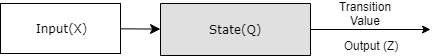
\includegraphics[scale=0.75]{Mealydiagram.png}
        \caption{\color{cyan}Mealy sate machine simple representation}
        \label{fig:ej1mealyr}
    \end{figure}

In this exercise, two sensors I and S function as input event to the state machine. Analyzing the possible states and event we obtain the following Mealy machine diagram:

 \begin{figure}[h!]
        \centering
        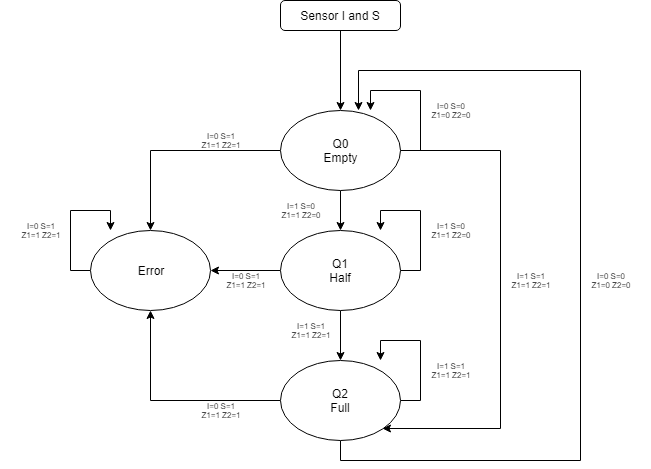
\includegraphics[scale=0.65]{ej1mealy.png}
        \caption{\color{cyan}Exercise 1: Mealy sate machine flow chart}
        \label{fig:ej1mealyd}
    \end{figure}

Which is represented as follow:

% Please add the following required packages to your document preamble:
% \usepackage{multirow}
\begin{table}[h!]
\centering
\begin{tabular}{|c|c|c|c|c|c|c|c|c|c|c|}
\hline
\multicolumn{3}{|c|}{\multirow{2}{*}{\textbf{State(Q)}}} & \multicolumn{8}{c|}{\textbf{Input(X)}} \\ \cline{4-11} 
\multicolumn{3}{|c|}{} & \multicolumn{2}{c|}{\textbf{I=0 S=0}} & \multicolumn{2}{c|}{\textbf{I=0 S=1}} & \multicolumn{2}{c|}{\textbf{I=1 S=0}} & \multicolumn{2}{c|}{\textbf{I=1 S=1}} \\ \hline
\textbf{Representation} & \textbf{Q2} & \textbf{Q1} & \textbf{Q2} & \textbf{Q1} & \textbf{Q2} & \textbf{Q1} & \textbf{Q2} & \textbf{Q1} & \textbf{Q2} & \textbf{Q1} \\ \hline
\textbf{Empty} & 0 & 0 & 0 & 0 & 0 & 1 & 1 & 0 & 1 & 1 \\ \hline
\textbf{Error} & 0 & 1 & 0 & 0 & 0 & 1 & 1 & 0 & 1 & 1 \\ \hline
\textbf{Half} & 1 & 0 & 0 & 0 & 0 & 1 & 1 & 0 & 1 & 1 \\ \hline
\textbf{Full} & 1 & 1 & 0 & 0 & 0 & 1 & 1 & 0 & 1 & 1 \\ \hline
\textbf{Output(Z)} & \textbf{Z1} & \textbf{Z2} & \textbf{0} & \textbf{0} & \textbf{1} & \textbf{1} & \textbf{1} & \textbf{0} & \textbf{1} & \textbf{1} \\ \hline
\end{tabular}
\caption{\color{cyan}Exercise 1: Mealy sate machine}
\end{table}

\pagebreak
So the logic circuit would be:

 \begin{figure}[h!]
        \centering
        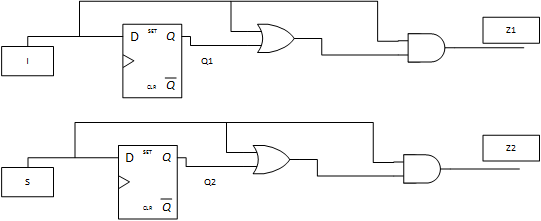
\includegraphics[scale=1]{ej1mealycircuit.png}
        \caption{\color{cyan}Exercise 1: Mealy logic circuit}
        \label{fig:ej1mealyld}
    \end{figure}

We can notice that the input event and the output event are the same which could make the $Z_N=X_N$ with N: the output or input number, but as mention be in the Mealy state machine the output $Z=f(X_1.....X_n,Q_1....Q_n)$, so we considered essential the use of sate in the circuit is dependent with the state and the input to have a clear view of being a Mealy state machine.

\subsubsection{\color{Orange}Simulation}

For the simulation of this stage machine, as the pump B1 and B2 alternate their function when $I = 1 y S = 0$ and for the activation of the pump that depends on output voltage is needed the following circuit is added:

 \begin{figure}[h!]
        \centering
        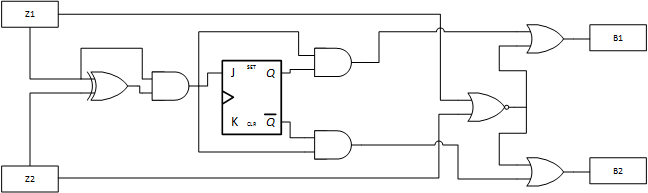
\includegraphics[scale=1]{ej1mealycircuitplus.png}
        \caption{\color{cyan}Exercise 1: Mealy additional logic circuit for the simulation}
        \label{fig:ej1mealylp}
    \end{figure}
    
Simulation the complete circuit in Verilog and testing the possibles values of input in Gtkwave the result was:

 \begin{figure}[h!]
        \centering
        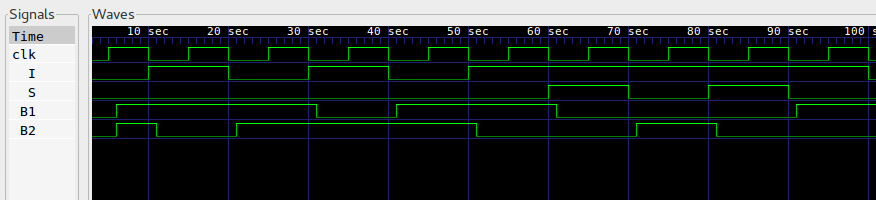
\includegraphics[scale=0.7]{ej1mealysim1.png}\\
        \vspace{0.2cm}
        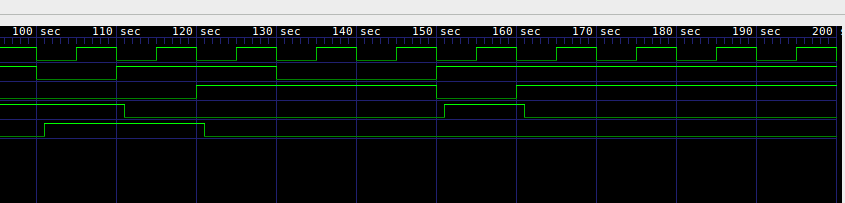
\includegraphics[scale=0.73]{ej1mealysim2.png}
        \caption{\color{cyan}Exercise 1: Simulation results}
        \label{fig:ej1mealyw}
    \end{figure}

%%%%%%%%%%%%%%%%%%%%%%%%%%%%%%%%%%%%%%%%
%Para Maleeeee
\pagebreak
Esto es Y1
\begin{center}
        \begin{Karnaugh}
            %cada 4 es una fila, la col 3 es la 4ta columna y 3fila es la 4 fila
            \contingut{
            0,0,1,0,
            0,X,X,X,
            1,0,0,0,
            0,X,X,X}
            \implicant{2}{6}{red}
            \implicant{8}{8}{green}
%            \implicant{12}{8}{orange}
%            \implicantdaltbaix[3pt]{1}{9}{blue}
            %\implicantcantons[2pt]{orange}
            %\implicantcostats{4}{14}{green}
        \end{Karnaugh}
    \end{center}

Y2
\begin{center}
        \begin{Karnaugh}
            %cada 4 es una fila, la col 3 es la 4ta columna y 3fila es la 4 fila
            \contingut{
            0,0,1,0,
            0,X,X,X,
            0,1,1,0,
            1,X,X,X}
            \implicant{2}{10}{red}
            \implicant{12}{14}{green}
%            \implicant{12}{8}{orange}
            \implicant{13}{9}{blue}
%            \implicantdaltbaix[3pt]{1}{9}{blue}
            %\implicantcantons[2pt]{orange}
            %\implicantcostats{4}{14}{green}
        \end{Karnaugh}
    \end{center}
  
  Y3  
\begin{center}
        \begin{Karnaugh}
            %cada 4 es una fila, la col 3 es la 4ta columna y 3fila es la 4 fila
            \contingut{
            0,0,0,0,
            0,X,X,X,
            0,0,0,1,
            0,X,X,X}
            \implicant{15}{11}{red}
%            \implicant{12}{14}{green}
%%            \implicant{12}{8}{orange}
%            \implicant{13}{9}{blue}
%            \implicantdaltbaix[3pt]{1}{9}{blue}
            %\implicantcantons[2pt]{orange}
            %\implicantcostats{4}{14}{green}
        \end{Karnaugh}
    \end{center}
    
    Z
    \begin{center}
        \begin{Karnaughvuit}
            %cada 4 es una fila, la col 3 es la 4ta columna y 3fila es la 4 fila
            \minterms{4}
        \maxterms{0,1,2,3}
        \indeterminats{5,6,7}
            \implicant{4}{6}{red}
%            \implicant{12}{14}{green}
%%            \implicant{12}{8}{orange}
%            \implicant{13}{9}{blue}
%            \implicantdaltbaix[3pt]{1}{9}{blue}
            %\implicantcantons[2pt]{orange}
            %\implicantcostats{4}{14}{green}
        \end{Karnaughvuit}
    \end{center}

%%%%%%%%%%%%%%%%%%%%%%%%%%%%%%%%%%%%%%%


\end{document}













\section{Design}
blabber.


%\newpage
\pagenumbering{roman}
\section{Appendix}

\begin{figure}[h!] %cambio la H por!
\begin{centering}
\includegraphics[scale=0.4]{../E4TP1/images/5}
\par\end{centering}
\caption{\color{cyan}Verilog implementation of Excercise 4}
\label{fig:figura4.6}
\end{figure}

\begin{figure}[h!]%cambio la H por!
\begin{centering}
\includegraphics[scale=0.4]{../E4TP1/images/6}
\par\end{centering}
\caption{\color{cyan}Terminal's output of Excercise 4}
\label{fig:figura4.7}
\end{figure}


%%% End document
\end{document}
%%% Preamble
\documentclass[paper=a4, fontsize=11pt]{scrartcl}

%%AGREG0
\usepackage{float}
%\usepackage{geometry}
%\geometry{verbose,tmargin=2cm,bmargin=2cm,lmargin=2cm,rmargin=2cm,headheight=2cm,headsep=2cm}
%\geometry{verbose,tmargin=2cm,bmargin=2cm,lmargin=2cm,rmargin=2cm,headheight=2cm,headsep=2cm}

\usepackage[T1]{fontenc}
\usepackage{fourier}
\usepackage[utf8]{inputenc}
\usepackage[english]{babel}					% English language/hyphenation

\usepackage[protrusion=true,expansion=true]{microtype}	
\usepackage{amsmath,amsfonts,amsthm} % Math packages
\usepackage[pdftex]{graphicx}	
\usepackage{url}
\usepackage{import}

\usepackage[margin=2cm]{geometry}
\geometry{verbose,tmargin=2cm,bmargin=2cm,lmargin=2cm,rmargin=2cm,headheight=2cm,headsep=2cm}
% %%% Custom sectioning
\usepackage{sectsty}
\allsectionsfont{\normalfont \scshape}


%%% Custom headers/footers (fancyhdr package)
\usepackage{fancyhdr}
\pagestyle{fancyplain}
\fancyhead{}											% No page header
\fancyfoot[L]{}											% Empty 
\fancyfoot[C]{}											% Empty
\fancyfoot[R]{\thepage}									% Pagenumbering
\renewcommand{\headrulewidth}{0pt}			% Remove header underlines
\renewcommand{\footrulewidth}{0pt}				% Remove footer underlines
\setlength{\headheight}{13.6pt}


%%% Equation and float numbering
\numberwithin{equation}{section}		% Equationnumbering: section.eq#
\numberwithin{figure}{section}			% Figurenumbering: section.fig#
\numberwithin{table}{section}				% Tablenumbering: section.tab#


%%% Maketitle metadata
\newcommand{\horrule}[1]{\rule{\linewidth}{#1}} 	% Horizontal rule

%AGREGO PARA EJ 1
\usepackage{graphicx}
\usepackage{color} 
\usepackage[dvipsnames]{xcolor}
\colorlet{purple}{purple}

%/////////////////////////////////// AGREGO PARA EL EJ 2

    \usepackage{geometry} % Required to change the page size to A4
    \geometry{a4paper} % Set the page size to be A4 as opposed to the default US Letter

    \usepackage{mathtools, nccmath}
    
    \usepackage{tikz}
    \usetikzlibrary{matrix,calc}

    %isolated term
%#1 - Optional. Space between node and grouping line. Default=0
%#2 - node
%#3 - filling color
\newcommand{\implicantsol}[3][0]{
    \draw[rounded corners=3pt, fill=#3, opacity=0.3] ($(#2.north west)+(135:#1)$) rectangle ($(#2.south east)+(-45:#1)$);
    }


%internal group
%#1 - Optional. Space between node and grouping line. Default=0
%#2 - top left node
%#3 - bottom right node
%#4 - filling color
\newcommand{\implicant}[4][0]{
    \draw[rounded corners=3pt, fill=#4, opacity=0.3] ($(#2.north west)+(135:#1)$) rectangle ($(#3.south east)+(-45:#1)$);
    }

%group lateral borders
%#1 - Optional. Space between node and grouping line. Default=0
%#2 - top left node
%#3 - bottom right node
%#4 - filling color
\newcommand{\implicantcostats}[4][0]{
    \draw[rounded corners=3pt, fill=#4, opacity=0.3] ($(rf.east |- #2.north)+(90:#1)$)-| ($(#2.east)+(0:#1)$) |- ($(rf.east |- #3.south)+(-90:#1)$);
    \draw[rounded corners=3pt, fill=#4, opacity=0.3] ($(cf.west |- #2.north)+(90:#1)$) -| ($(#3.west)+(180:#1)$) |- ($(cf.west |- #3.south)+(-90:#1)$);
}

%group top-bottom borders
%#1 - Optional. Space between node and grouping line. Default=0
%#2 - top left node
%#3 - bottom right node
%#4 - filling color
\newcommand{\implicantdaltbaix}[4][0]{
    \draw[rounded corners=3pt, fill=#4, opacity=0.3] ($(cf.south -| #2.west)+(180:#1)$) |- ($(#2.south)+(-90:#1)$) -| ($(cf.south -| #3.east)+(0:#1)$);
    \draw[rounded corners=3pt, fill=#4, opacity=0.3] ($(rf.north -| #2.west)+(180:#1)$) |- ($(#3.north)+(90:#1)$) -| ($(rf.north -| #3.east)+(0:#1)$);
}

%group corners
%#1 - Optional. Space between node and grouping line. Default=0
%#2 - filling color
\newcommand{\implicantcantons}[2][0]{
    \draw[rounded corners=3pt, opacity=.3] ($(rf.east |- 0.south)+(-90:#1)$) -| ($(0.east |- cf.south)+(0:#1)$);
    \draw[rounded corners=3pt, opacity=.3] ($(rf.east |- 8.north)+(90:#1)$) -| ($(8.east |- rf.north)+(0:#1)$);
    \draw[rounded corners=3pt, opacity=.3] ($(cf.west |- 2.south)+(-90:#1)$) -| ($(2.west |- cf.south)+(180:#1)$);
    \draw[rounded corners=3pt, opacity=.3] ($(cf.west |- 10.north)+(90:#1)$) -| ($(10.west |- rf.north)+(180:#1)$);
    \fill[rounded corners=3pt, fill=#2, opacity=.3] ($(rf.east |- 0.south)+(-90:#1)$) -|  ($(0.east |- cf.south)+(0:#1)$) [sharp corners] ($(rf.east |- 0.south)+(-90:#1)$) |-  ($(0.east |- cf.south)+(0:#1)$) ;
    \fill[rounded corners=3pt, fill=#2, opacity=.3] ($(rf.east |- 8.north)+(90:#1)$) -| ($(8.east |- rf.north)+(0:#1)$) [sharp corners] ($(rf.east |- 8.north)+(90:#1)$) |- ($(8.east |- rf.north)+(0:#1)$) ;
    \fill[rounded corners=3pt, fill=#2, opacity=.3] ($(cf.west |- 2.south)+(-90:#1)$) -| ($(2.west |- cf.south)+(180:#1)$) [sharp corners]($(cf.west |- 2.south)+(-90:#1)$) |- ($(2.west |- cf.south)+(180:#1)$) ;
    \fill[rounded corners=3pt, fill=#2, opacity=.3] ($(cf.west |- 10.north)+(90:#1)$) -| ($(10.west |- rf.north)+(180:#1)$) [sharp corners] ($(cf.west |- 10.north)+(90:#1)$) |- ($(10.west |- rf.north)+(180:#1)$) ;
}

%Empty Karnaugh map 4x4
\newenvironment{Karnaugh}%
{
\begin{tikzpicture}[baseline=(current bounding box.north),scale=0.8]
\draw (0,0) grid (4,4);
\draw (0,4) -- node [pos=0.7,above right,anchor=south west] {y2 y1} node [pos=0.75,below left,anchor=north east] {w y3} ++(135:1);
%
\matrix (mapa) [matrix of nodes,
        column sep={0.8cm,between origins},
        row sep={0.8cm,between origins},
        every node/.style={minimum size=0.3mm},
        anchor=8.center,
        ampersand replacement=\&] at (0.5,0.5)
{
                       \& |(c00)| 00         \& |(c01)| 01         \& |(c11)| 11         \& |(c10)| 10         \& |(cf)| \phantom{00} \\
|(r00)| 00             \& |(0)|  \phantom{0} \& |(1)|  \phantom{0} \& |(3)|  \phantom{0} \& |(2)|  \phantom{0} \&                     \\
|(r01)| 01             \& |(4)|  \phantom{0} \& |(5)|  \phantom{0} \& |(7)|  \phantom{0} \& |(6)|  \phantom{0} \&                     \\
|(r11)| 11             \& |(12)| \phantom{0} \& |(13)| \phantom{0} \& |(15)| \phantom{0} \& |(14)| \phantom{0} \&                     \\
|(r10)| 10             \& |(8)|  \phantom{0} \& |(9)|  \phantom{0} \& |(11)| \phantom{0} \& |(10)| \phantom{0} \&                     \\
|(rf) | \phantom{00}   \&                    \&                    \&                    \&                    \&                     \\
};
}%
{
\end{tikzpicture}
}

%Empty Karnaugh map 2x4
\newenvironment{Karnaughvuit}%
{
\begin{tikzpicture}[baseline=(current bounding box.north),scale=0.8]
\draw (0,0) grid (4,2);
\draw (0,2) -- node [pos=0.7,above right,anchor=south west] {y2 y1} node [pos=0.7,below left,anchor=north east] {y3} ++(135:1);
%
\matrix (mapa) [matrix of nodes,
        column sep={0.8cm,between origins},
        row sep={0.8cm,between origins},
        every node/.style={minimum size=0.3mm},
        anchor=4.center,
        ampersand replacement=\&] at (0.5,0.5)
{
                      \& |(c00)| 00         \& |(c01)| 01         \& |(c11)| 11         \& |(c10)| 10         \& |(cf)| \phantom{00} \\
|(r00)| 0             \& |(0)|  \phantom{0} \& |(1)|  \phantom{0} \& |(3)|  \phantom{0} \& |(2)|  \phantom{0} \&                     \\
|(r01)| 1             \& |(4)|  \phantom{0} \& |(5)|  \phantom{0} \& |(7)|  \phantom{0} \& |(6)|  \phantom{0} \&                     \\
|(rf) | \phantom{00}  \&                    \&                    \&                    \&                    \&                     \\
};
}%
{
\end{tikzpicture}
}

%Empty Karnaugh map 2x2
\newenvironment{Karnaughquatre}%
{
\begin{tikzpicture}[baseline=(current bounding box.north),scale=0.8]
\draw (0,0) grid (2,2);
\draw (0,2) -- node [pos=0.7,above right,anchor=south west] {b} node [pos=0.7,below left,anchor=north east] {a} ++(135:1);
%
\matrix (mapa) [matrix of nodes,
        column sep={0.8cm,between origins},
        row sep={0.8cm,between origins},
        every node/.style={minimum size=0.3mm},
        anchor=2.center,
        ampersand replacement=\&] at (0.5,0.5)
{
          \& |(c00)| 0          \& |(c01)| 1  \\
|(r00)| 0 \& |(0)|  \phantom{0} \& |(1)|  \phantom{0} \\
|(r01)| 1 \& |(2)|  \phantom{0} \& |(3)|  \phantom{0} \\
};
}%
{
\end{tikzpicture}
}

%Defines 8 or 16 values (0,1,X)
\newcommand{\contingut}[1]{%
\foreach \x [count=\xi from 0]  in {#1}
     \path (\xi) node {\x};
}

%Places 1 in listed positions
\newcommand{\minterms}[1]{%
    \foreach \x in {#1}
        \path (\x) node {1};
}

%Places 0 in listed positions
\newcommand{\maxterms}[1]{%
    \foreach \x in {#1}
        \path (\x) node {0};
}

%Places X in listed positions
\newcommand{\indeterminats}[1]{%
    \foreach \x in {#1}
        \path (\x) node {X};
}

    \linespread{1.2} % Line spacing
    
    \setlength\parindent{0pt} % Uncomment to remove all indentation from paragraphs
    
   % \graphicspath{{/home/bzerol/VisualCode/ElectroIII/tp1-team-2/E2TP1}} % Specifies the directory where pictures are stored

%//////////////////////////////////// agrego para EJ 4
%\documentclass[english]{article}
%\usepackage[T1]{fontenc}
%\usepackage[latin9]{inputenc}
%\usepackage{geometry}
%\geometry{verbose,tmargin=2cm,bmargin=2cm,lmargin=2cm,rmargin=2cm,headheight=2cm,headsep=2cm}
%\usepackage{float}
%\usepackage{graphicx}

\makeatletter

%%%%%%%%%%%%%%%%%%%%%%%%%%%%%% LyX specific LaTeX commands.
%% Because html converters don't know tabularnewline
\providecommand{\tabularnewline}{\\}

%%%%%%%%%%%%%%%%%%%%%%%%%%%%%% User specified LaTeX commands.
\usepackage{babel}


\makeatother

\usepackage{babel}

%///////////////////////////// PARA EL EJ6
%\documentclass[english]{article}
%\usepackage[T1]{fontenc}
%\usepackage[latin9]{inputenc}
%\usepackage{geometry}
%\geometry{verbose,tmargin=3cm,bmargin=3cm,lmargin=3cm,rmargin=3cm,headheight=3cm,headsep=3cm}
%\usepackage{float}

%\makeatletter

%%%%%%%%%%%%%%%%%%%%%%%%%%%%%% LyX specific LaTeX commands.
%% Because html converters don't know tabularnewline
\providecommand{\tabularnewline}{\\}



\begin{document}

%\begin{titlepage}
    
\newcommand{\HRule}{\rule{\linewidth}{0.5mm}} % Defines a new command for the horizontal lines, change thickness here
    
\center % Center everything on the page
     
%----------------------------------------------------------------------------------------
%	HEADING SECTIONS
%----------------------------------------------------------------------------------------
    
\textsc{\LARGE Instituto Tecnológico de Buenos Aires}\\[2cm] % Name of your university/college
\textsc{\Large Electronica III}\\[1.5cm] % Major heading such as course name
\textsc{\large Trabajo Práctico N° 3}\\[0.5cm] % Minor heading such as course title
    
%----------------------------------------------------------------------------------------
%	TITLE SECTION
%----------------------------------------------------------------------------------------
    
\HRule \\[0.5cm]
{ \huge \bfseries Trabajo Práctico de Laboratorio Nr. 3}\\[0.4cm] % Title of your document
\HRule \\[2cm]
     
%----------------------------------------------------------------------------------------
%	AUTHOR SECTION
%----------------------------------------------------------------------------------------
    
\begin{minipage}{0.4\textwidth}
\begin{flushleft} \large
\emph{Grupo 2:}\\		%names
[.3cm]
Victor \textsc{Oh}\\
Leg. ???\\ 
[.3cm]
Ian \textsc{Diaz}\\
Leg. ???\\ 
[.3cm]
Benjamín Carlos \textsc{Lin}\\
Leg. 57242 \\ 
[.3cm]
Malena \textsc{Muller}\\
Leg. ???\\ 
[.3cm]
\end{flushleft}
\end{minipage}
~
\begin{minipage}{0.4\textwidth}
\begin{flushright} \large
%\emph{Profesor:} \\
%[.3cm]
%Pablo  \textsc{Cossutta}\\ % Supervisor's Name
%Alejandra \textsc{Weill} \\% Supervisor's Name
%Matías  \textsc{Salvati} % Supervisor's Name
\end{flushright}
\end{minipage}\\[2cm]
    
%----------------------------------------------------------------------------------------
%	DATE SECTION
%----------------------------------------------------------------------------------------
    
\vfill
{\large Entregado: 17 de Octubre de 2018}\\[2cm]
    
\vfill 
    
\end{titlepage}
%
%\pagenumbering{roman}
%\tableofcontents
%\newpage
%\pagenumbering{arabic}
%
%Test Text

\section{\color{olive}Exercise 1: Tank simulation}

\subsection{\color{purple}Mealy State Machine}

In the Mealy state machine, the output value not only depends on the state we are but also depends on the input values. This is to say the output could be represented as a function like $Z=f(X_1.....X_n,Q_1....Q_n)$ where Z: output, Q: State and X:Input event as could be visualize:

 \begin{figure}[h!]
        \centering
        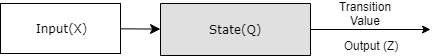
\includegraphics[scale=0.75]{Mealydiagram.png}
        \caption{\color{cyan}Mealy sate machine simple representation}
        \label{fig:ej1mealyr}
    \end{figure}

In this exercise, two sensors I and S function as input event to the state machine. Analyzing the possible states and event we obtain the following Mealy machine diagram:

 \begin{figure}[h!]
        \centering
        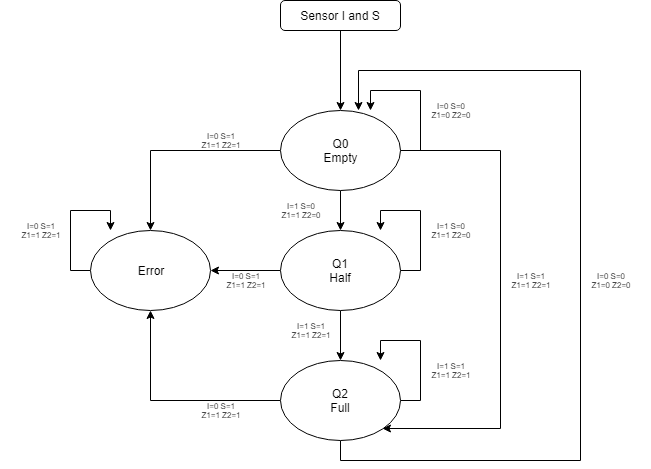
\includegraphics[scale=0.65]{ej1mealy.png}
        \caption{\color{cyan}Exercise 1: Mealy sate machine flow chart}
        \label{fig:ej1mealyd}
    \end{figure}

Which is represented as follow:

% Please add the following required packages to your document preamble:
% \usepackage{multirow}
\begin{table}[h!]
\centering
\begin{tabular}{|c|c|c|c|c|c|c|c|c|c|c|}
\hline
\multicolumn{3}{|c|}{\multirow{2}{*}{\textbf{State(Q)}}} & \multicolumn{8}{c|}{\textbf{Input(X)}} \\ \cline{4-11} 
\multicolumn{3}{|c|}{} & \multicolumn{2}{c|}{\textbf{I=0 S=0}} & \multicolumn{2}{c|}{\textbf{I=0 S=1}} & \multicolumn{2}{c|}{\textbf{I=1 S=0}} & \multicolumn{2}{c|}{\textbf{I=1 S=1}} \\ \hline
\textbf{Representation} & \textbf{Q2} & \textbf{Q1} & \textbf{Q2} & \textbf{Q1} & \textbf{Q2} & \textbf{Q1} & \textbf{Q2} & \textbf{Q1} & \textbf{Q2} & \textbf{Q1} \\ \hline
\textbf{Empty} & 0 & 0 & 0 & 0 & 0 & 1 & 1 & 0 & 1 & 1 \\ \hline
\textbf{Error} & 0 & 1 & 0 & 0 & 0 & 1 & 1 & 0 & 1 & 1 \\ \hline
\textbf{Half} & 1 & 0 & 0 & 0 & 0 & 1 & 1 & 0 & 1 & 1 \\ \hline
\textbf{Full} & 1 & 1 & 0 & 0 & 0 & 1 & 1 & 0 & 1 & 1 \\ \hline
\textbf{Output(Z)} & \textbf{Z1} & \textbf{Z2} & \textbf{0} & \textbf{0} & \textbf{1} & \textbf{1} & \textbf{1} & \textbf{0} & \textbf{1} & \textbf{1} \\ \hline
\end{tabular}
\caption{\color{cyan}Exercise 1: Mealy sate machine}
\end{table}

\pagebreak
So the logic circuit would be:

 \begin{figure}[h!]
        \centering
        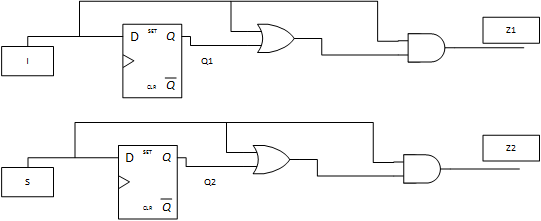
\includegraphics[scale=1]{ej1mealycircuit.png}
        \caption{\color{cyan}Exercise 1: Mealy logic circuit}
        \label{fig:ej1mealyld}
    \end{figure}

We can notice that the input event and the output event are the same which could make the $Z_N=X_N$ with N: the output or input number, but as mention be in the Mealy state machine the output $Z=f(X_1.....X_n,Q_1....Q_n)$, so we considered essential the use of sate in the circuit is dependent with the state and the input to have a clear view of being a Mealy state machine.

\subsubsection{\color{Orange}Simulation}

For the simulation of this stage machine, as the pump B1 and B2 alternate their function when $I = 1 y S = 0$ and for the activation of the pump that depends on output voltage is needed the following circuit is added:

 \begin{figure}[h!]
        \centering
        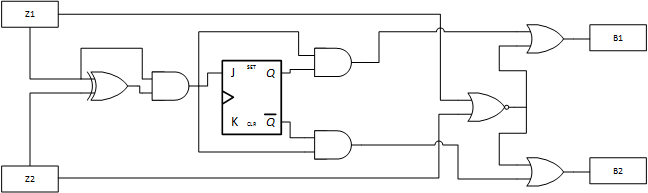
\includegraphics[scale=1]{ej1mealycircuitplus.png}
        \caption{\color{cyan}Exercise 1: Mealy additional logic circuit for the simulation}
        \label{fig:ej1mealylp}
    \end{figure}
    
Simulation the complete circuit in Verilog and testing the possibles values of input in Gtkwave the result was:

 \begin{figure}[h!]
        \centering
        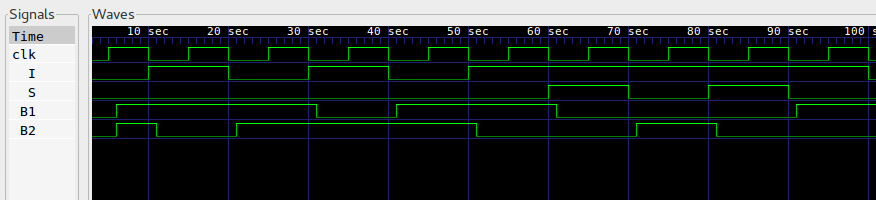
\includegraphics[scale=0.7]{ej1mealysim1.png}\\
        \vspace{0.2cm}
        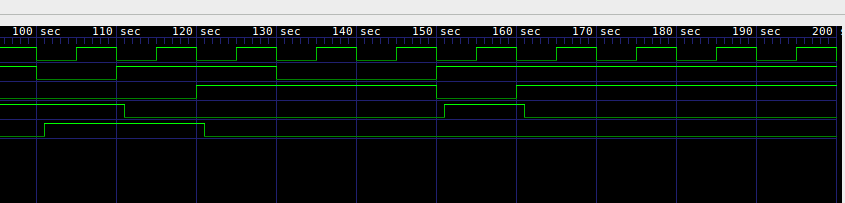
\includegraphics[scale=0.73]{ej1mealysim2.png}
        \caption{\color{cyan}Exercise 1: Simulation results}
        \label{fig:ej1mealyw}
    \end{figure}

%%%%%%%%%%%%%%%%%%%%%%%%%%%%%%%%%%%%%%%%
%Para Maleeeee
\pagebreak
Esto es Y1
\begin{center}
        \begin{Karnaugh}
            %cada 4 es una fila, la col 3 es la 4ta columna y 3fila es la 4 fila
            \contingut{
            0,0,1,0,
            0,X,X,X,
            1,0,0,0,
            0,X,X,X}
            \implicant{2}{6}{red}
            \implicant{8}{8}{green}
%            \implicant{12}{8}{orange}
%            \implicantdaltbaix[3pt]{1}{9}{blue}
            %\implicantcantons[2pt]{orange}
            %\implicantcostats{4}{14}{green}
        \end{Karnaugh}
    \end{center}

Y2
\begin{center}
        \begin{Karnaugh}
            %cada 4 es una fila, la col 3 es la 4ta columna y 3fila es la 4 fila
            \contingut{
            0,0,1,0,
            0,X,X,X,
            0,1,1,0,
            1,X,X,X}
            \implicant{2}{10}{red}
            \implicant{12}{14}{green}
%            \implicant{12}{8}{orange}
            \implicant{13}{9}{blue}
%            \implicantdaltbaix[3pt]{1}{9}{blue}
            %\implicantcantons[2pt]{orange}
            %\implicantcostats{4}{14}{green}
        \end{Karnaugh}
    \end{center}
  
  Y3  
\begin{center}
        \begin{Karnaugh}
            %cada 4 es una fila, la col 3 es la 4ta columna y 3fila es la 4 fila
            \contingut{
            0,0,0,0,
            0,X,X,X,
            0,0,0,1,
            0,X,X,X}
            \implicant{15}{11}{red}
%            \implicant{12}{14}{green}
%%            \implicant{12}{8}{orange}
%            \implicant{13}{9}{blue}
%            \implicantdaltbaix[3pt]{1}{9}{blue}
            %\implicantcantons[2pt]{orange}
            %\implicantcostats{4}{14}{green}
        \end{Karnaugh}
    \end{center}
    
    Z
    \begin{center}
        \begin{Karnaughvuit}
            %cada 4 es una fila, la col 3 es la 4ta columna y 3fila es la 4 fila
            \minterms{4}
        \maxterms{0,1,2,3}
        \indeterminats{5,6,7}
            \implicant{4}{6}{red}
%            \implicant{12}{14}{green}
%%            \implicant{12}{8}{orange}
%            \implicant{13}{9}{blue}
%            \implicantdaltbaix[3pt]{1}{9}{blue}
            %\implicantcantons[2pt]{orange}
            %\implicantcostats{4}{14}{green}
        \end{Karnaughvuit}
    \end{center}

%%%%%%%%%%%%%%%%%%%%%%%%%%%%%%%%%%%%%%%


\end{document}













%EXCERCISE 1 :)

\section{\color{olive}Excercise 2: State Machines to Detect the sequence 1-1-0-1}
In this exercise, the detection of the sequence 1-1-0-1 inside a longer sequence of bits, is done with a Moore's state machine and with a Mealy's state machine. The main difference between these two state machines is that in Moore's one, the output only depends on the present state of the machine, while in Mealy's one, the output depends on the present state as well as on the input. This causes a time displacement between the output of both state machines. Moore's output "answers" to the input one clock later after having reached the new state, while Mealy's output "answers" immediatly during the same clock that the input arrives. This is because Mealy's reacts not only according to the present state, but also depending on the input's value.

For the implementation of both state machines, five states are needed and they are represented with the letters A to E:
- A: "IDLE", the state in which the first digit of the sequence has not yet been detected.
- B: The first digit of the sequence, "1", has arrived.
- C: The second digit of the sequence, "1",  has arrived.
- D: The third digit of the sequence, "0", has arrived.
- E: The last digit of the sequence, "1", has arrived.

It is important to mention that no matter which is the present state, whenever a reset in "0" arrives,

\subsection{\color{purple}Moore Type State Machine}




\subsection{\color{purple}Mealy Type State Machine}



\section{\color{olive}Exercise 3}

For this exercise we were asked to implement the Moore machine shown
on Figure \ref{3_1}, but with one condition, everything inside our
machine should work on 3.3v and inputs and outputs should work on
5v logic.

\begin{figure}[H]
\begin{centering}
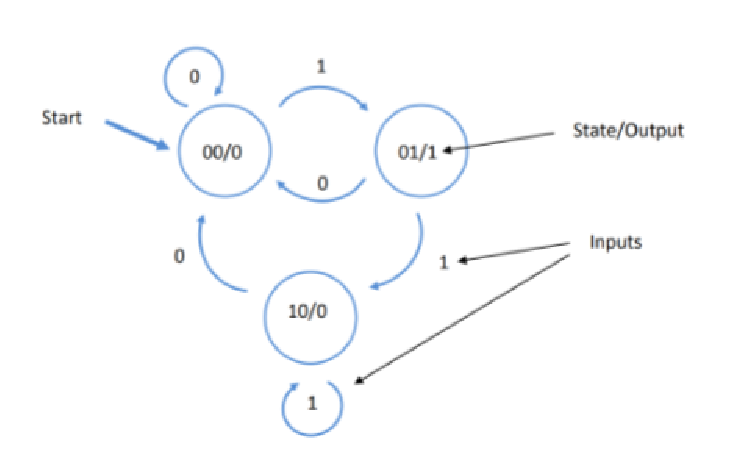
\includegraphics[scale=0.7]{../Exercise3/Assignment/images/Diagram}
\par\end{centering}
\caption{Moore Machine}
\label{3_1}
\end{figure}

\subsection{\color{purple}State Machine Implementation}

We proceeded to convert the diagram to a table that represents it,
and we got Table \ref{3_t_1}, and by transforming each bit (Output,
and next states bits) into a truth table, we could create our logic
implementation for each bit. The Truth Tables are shown on Tables
\ref{3_t_2}.

\begin{table}[H]
\begin{centering}
\begin{tabular}{|c|c|c|c|}
\hline 
State & W=0 & W=1 & Output\tabularnewline
\hline 
\hline 
00 & 00 & 01 & 0\tabularnewline
\hline 
01 & 00 & 10 & 1\tabularnewline
\hline 
10 & 00 & 10 & 0\tabularnewline
\hline 
\end{tabular}
\par\end{centering}
\caption{Moore Machine Table}
\label{3_t_1}

\end{table}

\begin{table}[H]
\begin{centering}
\begin{tabular}{|c|c|}
\hline 
S1 S0 & Output\tabularnewline
\hline 
\hline 
00 & 0\tabularnewline
\hline 
01 & 1\tabularnewline
\hline 
10 & 0\tabularnewline
\hline 
11 & x\tabularnewline
\hline 
\end{tabular} ~%
\begin{tabular}{|c|c|c|c|c|}
\hline 
S1 & S0 & W & S1' & S0'\tabularnewline
\hline 
\hline 
0 & 0 & 0 & 0 & 0\tabularnewline
\hline 
0 & 0 & 1 & 0 & 1\tabularnewline
\hline 
0 & 1 & 0 & 0 & 0\tabularnewline
\hline 
0 & 1 & 1 & 1 & 0\tabularnewline
\hline 
1 & 0 & 0 & 0 & 0\tabularnewline
\hline 
1 & 0 & 1 & 1 & 0\tabularnewline
\hline 
1 & 1 & 0 & x & x\tabularnewline
\hline 
1 & 1 & 1 & x & x\tabularnewline
\hline 
\end{tabular}
\par\end{centering}
\caption{Truth Tables}
\label{3_t_2}

\end{table}

So by re-writing those truth tables we have got the following equations:

\begin{equation}
Output=S_{1}\,.\,\bar{S_{0}}\label{eq:3_1}
\end{equation}

\[
S_{1}^{'}=\bar{S_{1}}S_{0}w+S_{1}\bar{S_{0}}w
\]

\[
S_{0}^{'}=\bar{S_{1}}\bar{S_{0}}w
\]

So, by implementing those formulas into a synchronized logic circuit,
we have got the Moore machine.

\subsection{\color{purple}Level Converter Implementation}

To convert the voltage levels on the PCB for compatibility, we decided
to use 2N7000 Mosfet Transistor. We used it to implement an inverter
with Open-Collector. By connecting the output to a pull-up network
with the voltage we want, we can convert the level with no problems,
form 5(v) to 3.3(v), and vice versa.

For the Pull-Up network, we decided to use a resistor $R=1\,(k\Omega)$
so that when it's conected to ground, te current flowing through the
inverter is less than $10\,(mA)$, and when the inverter produces
a High Z, the resistor its not enough big to produce a High Z to the
output, and set the output to a logic 1.

\subsection{\color{purple}PCB Implementation}

We proceeded to implement the PCB using Altium Designer, the Schematic
for this Finite State Machine is shown on Figure \ref{3_2}. The Top
and Bottom Layers are shown on Figure \ref{3_3}.

\begin{figure}[H]
\begin{centering}
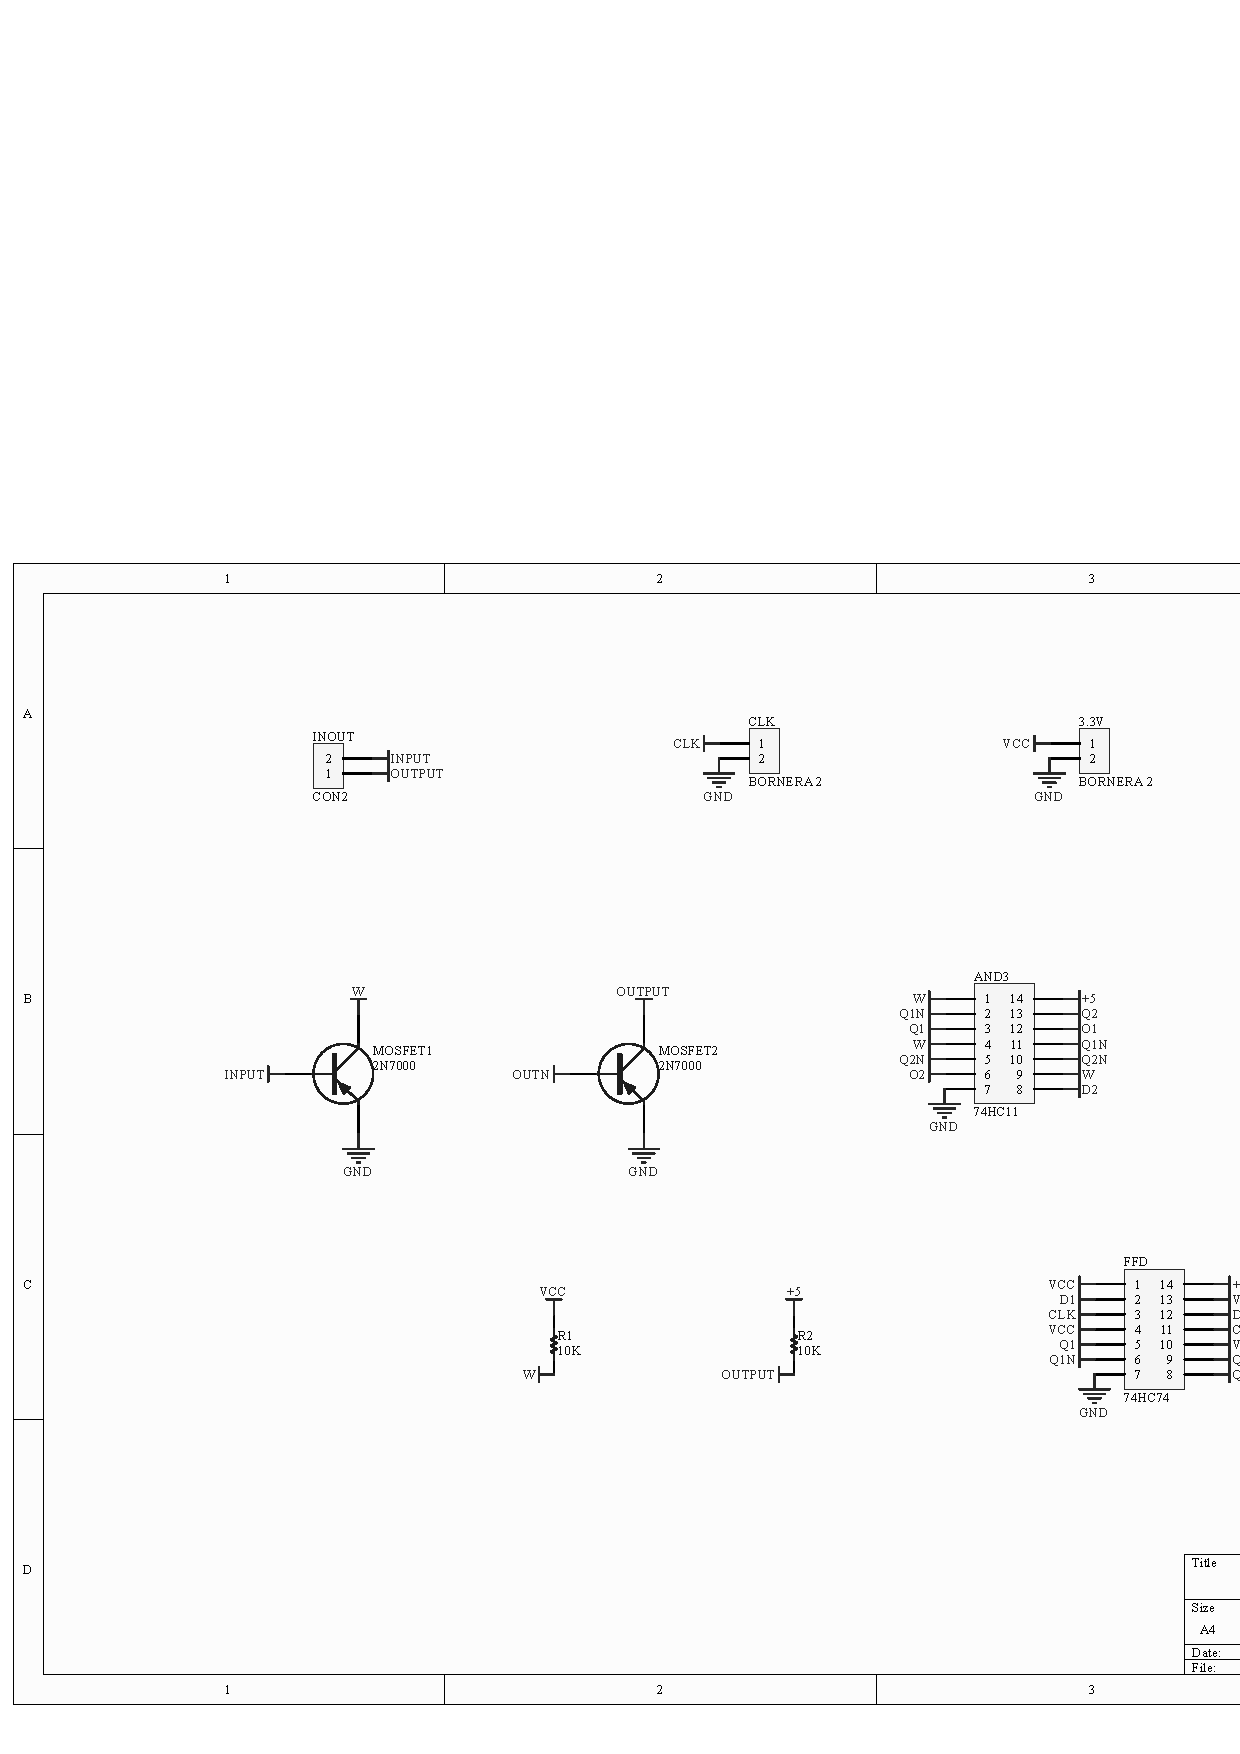
\includegraphics[scale=0.5]{../Exercise3/Assignment/images/Schematic}
\par\end{centering}
\caption{Schematic}
\label{3_2}

\end{figure}

\begin{figure}[H]
\begin{centering}
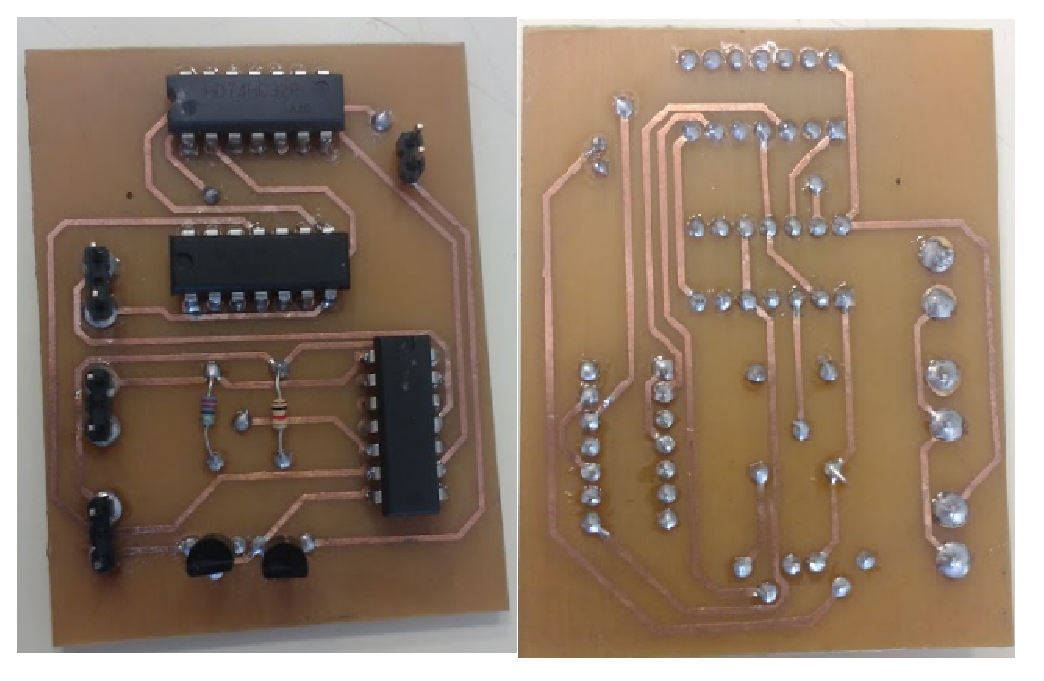
\includegraphics[scale=0.3]{../Exercise3/Assignment/images/TB}
\par\end{centering}
\caption{Printed Board}
\label{3_3}

\end{figure}

\subsection{\color{purple}Mealy State Machine Re-Implementation}

Finally, we were asked to re-implement the Moore State machine described
in the previous Subsections, into a Mealy State Machine. As we know,
Mealy Machines Outputs depend on states and inputs, different from
Moore that only depends on states. So the truth tables for the next
state, mantains its form and formula as the moore state machine, however,
the output truth table, and by consequence, its formula , change ash
shown on Table \ref{3_t_3}.

\begin{table}[H]
\begin{centering}
\begin{tabular}{|c|c|c|}
\hline 
State & W=0 & W=1\tabularnewline
\hline 
\hline 
00 & 00/0 & 01/1\tabularnewline
\hline 
01 & 00/0 & 10/0\tabularnewline
\hline 
10 & 00/0 & 10/0\tabularnewline
\hline 
\end{tabular}
\par\end{centering}
\caption{Mealy State Machine}
\label{3_t_4}
\end{table}

We can now easily see that in Table \ref{3_t_4}, states 01 and 10
are equal, so we can simplify those states into only one state. The
final Table is shown on Table \ref{3_t_5}.

\begin{table}[H]
\begin{centering}
\begin{tabular}{|c|c|c|}
\hline 
State & W=0 & W=1\tabularnewline
\hline 
\hline 
0 & 0/0 & 1/1\tabularnewline
\hline 
1 & 0/0 & 1/0\tabularnewline
\hline 
\end{tabular}
\par\end{centering}
\caption{Mealy Machine simplified}

\label{3_t_5}
\end{table}

\begin{table}[H]
\begin{centering}
\begin{tabular}{|c|c|c|}
\hline 
State & W & Output\tabularnewline
\hline 
\hline 
0 & 0 & 0\tabularnewline
\hline 
0 & 1 & 1\tabularnewline
\hline 
1 & 0 & 0\tabularnewline
\hline 
1 & 1 & 0\tabularnewline
\hline 
\end{tabular}
\par\end{centering}
\caption{Output Truth Table}

\label{3_t_3}
\end{table}

Finally, the formulas for the output and the next states are the following:

\[
Output=\bar{St}.W
\]

\[
State=W
\]

Implementing this would become someting like shown on Figure \ref{3_4}.

\begin{figure}[H]
\begin{centering}
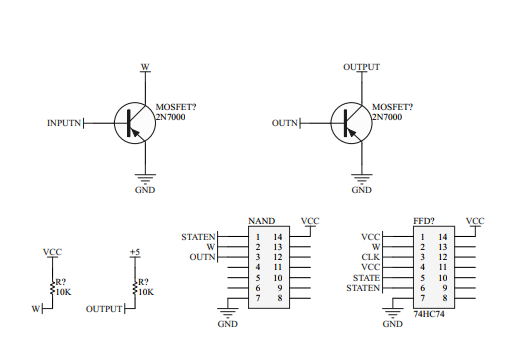
\includegraphics[scale=0.6]{../Exercise3/Assignment/images/Schematic2}
\par\end{centering}
\caption{Schematic Mealy Machine}
\label{3_4}

\end{figure}

We builded this schematic in a breadboard, as shon on Figure \ref{3_5}.

\begin{figure}[H]
\begin{centering}
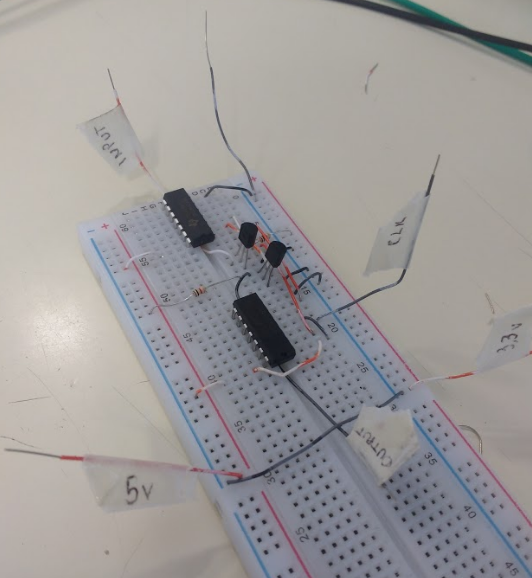
\includegraphics[scale=0.5]{../Exercise3/Assignment/images/mealy}
\par\end{centering}
\caption{Mealy Implementation}

\label{3_5}

\end{figure}

\subsection{\color{purple}Conclusions}

By analizing the behaviour of both circuits, how they behave in the
same test conditions, and comparing the amount of components used
in both PCBs, we conclude that in this case, Mealy's implementation
is more efficient because it utilizes less components and realizes
the same operation. However, we need to clarify that not always Mealy's
implementation is more efficient than Moore's, this depends on each
state machine to implement.
%\end{document}



%\newpage
\pagenumbering{roman}
\section{Appendix}

\begin{figure}[h!] %cambio la H por!
\begin{centering}
\includegraphics[scale=0.4]{../E4TP1/images/5}
\par\end{centering}
\caption{\color{cyan}Verilog implementation of Excercise 4}
\label{fig:figura4.6}
\end{figure}

\begin{figure}[h!]%cambio la H por!
\begin{centering}
\includegraphics[scale=0.4]{../E4TP1/images/6}
\par\end{centering}
\caption{\color{cyan}Terminal's output of Excercise 4}
\label{fig:figura4.7}
\end{figure}


%%% End document
\end{document}
